\documentclass[11pt,a4paper]{article}
\usepackage{times,latexsym}
\usepackage{url}
\usepackage[T1]{fontenc}
\usepackage[nohyperref]{tacl2021v1}
\usepackage{etoolbox}
\usepackage[hidelinks=true]{hyperref}
\usepackage{appendix}
\usepackage{natbib}
\usepackage[utf8x]{inputenc}
\usepackage{booktabs}
%\setlength {\marginparwidth }{2cm}
\usepackage{todonotes}
\usepackage{adjustbox}
\usepackage{microtype}
\usepackage{multirow}
\usepackage{placeins}
\usepackage{longtable}
\usepackage{enumitem}
\usepackage{amsmath}
\usepackage{cleveref}
\usepackage{wrapfig}
\usepackage{breqn}
\DeclareMathOperator*{\mean}{mean}
%%%%%%%%%%%%%%%%%%%%%%%%%%%%%%%%%%%%%%%%%%%%%%%%%%%%%%%%

\begin{document}

\title{Learning English with Peppa Pig}

\author{Mitja Nikolaus\\
  Aix-Marseille University\\
  \texttt{mitja.nikolaus@univ-amu.fr}
  \And
  Afra Alishahi\\
  Tilburg University\\
  \texttt{a.alishahi@uvt.nl}
  \And
  Grzegorz Chrupała\\
  Tilburg University\\
  \texttt{grzegorz@chrupala.me}}

\date{}


\maketitle
\begin{abstract}
  Attempts to computationally model or simulate the acquisition of
  spoken language via grounding in the visual modality have a long
  tradition but have gained momentum since around 2015 with the
  revival of neural networks. Current neural approaches are able to
  spot associations between the spoken and visual modality, and use
  these to represent speech and image/video data in a joint vector
  space. A major limitation of these works are the datasets used to
  train them. Most consist of static images or videos paired with
  spoken descriptions of what is depicted, and thus guarantee a strong
  correlation between speech and the visual world by construction. A
  child learning a language faces a very different and harder task: in
  the real world the coupling between the linguistic and the visual is
  much looser, and often contains confounds in the form of
  correlations with non-semantic aspects of the speech signal, such as
  voices of specific people and environmental sounds. The current
  study is a first step towards simulating such a naturalistic
  grounding scenario by using a dataset based on the children's
  cartoon {\it Peppa Pig}. We train a simple bi-modal architecture on
  the portion of the data consisting of naturalistic dialog between
  characters, and evaluate on segments containing descriptive
  narrations. Evaluation and analysis results indicate that despite
  the weak and confounded signal in this training data our model
  succeeds at learning aspects of the visual semantics of spoken
  language.
\end{abstract}

\section{Introduction}
\label{sec:intro}

Attempts to model or simulate the acquisition of spoken language via
grounding in the visual modality date to the beginning of this century
\citep{roypentland2002learning} but have gained momentum recently
with the revival of neural networks
\citep[e.g.][]{synnaeve2014learning,harwath2015deep,
  harwath2016unsupervised,chrupala-etal-2017-representations,alishahi-etal-2017-encoding,harwath2018jointly,Merkx2019,havard2019models,rouditchenko2020avlnet,khorrami_2021,peng2021fastslow}.
Current approaches work well enough from an applied point of view, 
but most are not generalizable to real-life situations that humans or 
adaptive artificial agents experience.Training data
typically consist of images or videos paired with spoken descriptions
of the scene depicted. The type of input that a language learner receives 
from its environment is much more challenging.  Firstly, speech is only
loosely coupled with the visual modality. Secondly in addition to
correlations between the visual scenes and the {\it meaning} of spoken
utterances, there are also correlations with non-semantic aspects of
the speech signal, such as the voice of specific speakers, as well
as with non-speech ambient sounds. Although it is plausible that such
non-semantic correlations can sometimes be useful to the learner in
the general endeavour of making sense of the world, for the specific
task of learning the semantics of linguistic units they are likely more
often an obstacle, as they make it harder to zoom in on the
meaning-bearing aspects of the audio signal.

In the current study we make a first step towards simulating the
acquisition of language via grounding in perception in a more naturalistic
scenario.  Our main focus is on learning the meaning of individual words 
as well as multi-word expressions from spoken utterances grounded in video.  
We use the well-known children's cartoon {\it Peppa Pig} as
a case study as a source of training and evaluation data. Compared to
commonly used video datasets, this data has a number of interesting
characteristics.  The visual modality is very schematic, and the
language is also simple in terms of vocabulary size and syntactic
complexity. Crucially, however, most of the speech in the videos
consists of naturalistic dialogs between the characters. The
utterances are only loosely and noisily correlated to the scenes and
actions depicted in the videos.\todo{GC: Can we support this assertion
  in a quantitative way? MN: Difficult I think. To measure semantic correlation 
  between images/videos and speech we need to pass them through a model. So we 
  could run our model on a different dataset (e.g. spoken captions) and show 
  that it performs better there, but we wouldn't have directly comparable 
  evaluation metrics..}

This choice of data thus allows us to directly address the ecological limitations 
of the current approaches. In addition, the cartoon videos also contain 
comments interjected by the narrator. We use these for a evaluation of the 
acquisition of meaning as they are more descriptive and less noisy and allow 
us to measure performance while controlling for speaker characteristics.
Our contributions are the following:
\begin{itemize}
\item We implement a simple bi-modal architecture which learns
  spoken language embeddings from videos;
\item We evaluate model performance in terms of video fragment
  retrieval and additionally design controlled evaluation
  protocols inspired by the intermodal preferential looking
  paradigm \citep{hirsh1996intermodal};
\item We carry out ablations of model components in order to
  understand the effects of pre-training for the audio and video
  encoders, the role of temporal information, and of segmentation
  strategies while training. 
\end{itemize}
We show that despite the challenges of our naturalistic training data
our model succeeds at learning robust associations between spoken 
forms and their visual semantics.
%aspects the visual semantics of spoken language. 
Our findings include the fact that temporal information
contributes substantially to video modeling, and that unsupervised
pre-training of the audio encoder is key to the best performance, but that
even the model trained completely from scratch on about 10 hours of
cartoon data performs substantially above chance.




\section{Related Work}
\label{sec:related}

Early attempts at simulating grounded language learning focus on
interactions between adults and young children while playing with a
set of objects from different categories \cite{roy1999learning,roy2002learning,
  gorniak2003visually,mukherjee2003visual}. In a representative study
from this series, \citet{roypentland2002learning} use speech recorded from
such interactions paired with different views of the visible objects
to identify linguistic units (i.e.\ words) and visual categories, and
to map these two modalities together. A hard-coded visual system
extracts object representations from images, and spoken utterances are
represented as phoneme probabilities generated by an RNN pre-trained on
spectrograms.  Their experiments on small-scale data (around 20 words
and seven visual categories) show that the model can segment words and
map them to visual categories.

\subsection{Spoken Language Grounded in Images}
\label{sec:images}
The availability of datasets of images associated with spoken captions
such as Flickr Audio Captions \cite{harwath2015deep}, Places
\cite{zhou2014learning} and Spoken COCO \cite{hsu2019transfer} led to
a rapid development of deep models of grounded language learning; see
\citet{chrupala-visually-2021} for a comprehensive overview. In contrast to 
earlier approaches, these models are trained end-to-end directly on large-scale 
raw input data.
Following the architecture proposed in \citet{karpathy2014deep} the visual and 
speech modality are usually encoded using separate pathways, and subsequently 
mapped into a joint representation space.
Visual features are extracted from a pre-trained
image classification model that processes the whole or a specific
region of an image (however see \citet{harwath2018jointly}, who train the
model end-to-end on images and their spoken captions on the Places
dataset). The audio encoder component in most models is 
either an adaptation of \citet{harwath2016unsupervised} which feeds a
spectrogram of the speech signal to a convolutional architecture, or a
hybrid architecture of convolutional followed by recurrent layers using
Mel-Frequency Cepstral Coefficient (MFCC) features from the audio
signal as input as introduced by \citet{chrupala-etal-2017-representations}.

Models of speech grounded in images are optimized for and evaluated on
image retrieval from spoken caption and vice versa. Additionally, a range of
diagnostic analyses have been performed on the hidden
representations of these models to study whether they encode 
the identity and boundaries of subword units such as phonemes
and syllables \cite{alishahi-etal-2017-encoding, harwath2019towards,
  khorrami_2021} as well as individual words
\cite{chrupala-etal-2017-representations,havard2019word}. Moreover, in
addition to examining form-meaning associations at the utterance
level, \citet{harwath-glass-2017-learning} explicitly learn a lexicon by
extracting audio and image segments, clustering each modality
separately, and mapping them together by calculating the pairwise
similarities of their members in the joint semantic space.

\subsection{Spoken Language Grounded in Video}
\label{sec:video}
There have also been recent attempts to learn spoken language grounded
in video instead of static images.  \citet{boggust2019grounding}
sample audio-visual fragments from cooking videos, however their
grounded model treats video frames as still images and discards their
temporal order.
% The loose synchrony between the two modalities, such that objects
% may be mentioned in the audio at a different point in time than they
% occur in the video, remains the main challenge for this approach.
\citet{rouditchenko2020avlnet} integrate the temporal information when
encoding videos from the Howto100m dataset \cite{miech2019howto100m},
and perform better than previous work in language and video clip
retrieval.
% Rouditchenko et al. (2021) present an architecture (AVLNet) which
% does model the time dimension in the video stream: the network
% consists of an audio encoder (ResNet-based), a video encoder which
% combines 3D and 2D modeling (also ResNet-based), as well as an
% optional text encoder.  This architecture is trained with a
% contrastive loss on randomly sampled audio-video fragments from the
% Howto100m dataset (Miech et al., 2019) consisting of 136 million
% video clips sourced from 1.22 million narrated instructional web
% videos. The model is evaluated on the video clip and language
% retrieval tasks on smaller video datasets annotated with clip
% boundaries and text summaries, and is shown to outperform previously
% proposed models of Arandjelovic and Zisserman (2018) and Boggust et
% al. (2019). The model also transfers to the image-audio retrieval
% setting. Qualitative analysis suggests that the model aligns
% semantically related audio and visual features to particular
% dimensions of the embedding space

Models trained on instructional video datasets often do not
generalize well to other domains. \citet{monfort2021spokenmoments}
highlight this limitation and show that training on their larger and
more diverse Spoken Moments in Time dataset leads to better
generalization.  But the point remains that these video datasets contain
descriptive speech, thus ensuring that there is a strong correlation
between the spoken language and their visual context, a characteristic
that is not representative of the experience of learning language in
 real world. We remedy this limitation by using a video dataset that does 
 not guarantee a direct description of the visual context. 

\subsection{Child Language Learning from Video}
% \todo[inline]{I'm still cleaning up the section on infant language
% learning from video.}  In addition to anecdotes and news pieces on
% how watching cartoons affects chidlren's accent and
% vocabulary\footnote{Example of stories on how watching Peppa Pig has
% changed children's accent and word usage:
% \url{https://www.theguardian.com/tv-and-radio/2021/jul/19/peppa-pig-american-kids-british-accents},
% \url{https://globalnews.ca/news/4961058/kids-accent-peppa-pig}.},
There are many studies on young children learning language by watching
videos; see \citet{vanderplank2010deja} for a survey. The main takeaway
of these studies is that language learning is much more effective in a
social, conversational setting than by passively watching videos
\cite{kuhl2003foreign,anderson2005television,robb2009just},
%\footnote{Adding
%social interaction while watching videos improves learning;
%\citet{lytle2018two}.} 
but learning does happen in such
contexts. Importantly for our goal, techniques such as the intermodal
preferential looking paradigm have been developed to systematically test young 
language learners' knowledge of words, syntactic structure and semantic roles
\cite{hirsh1996intermodal,bergelson20126,noble2011comprehension}.
\citet{nikolaus-fourtassi-2021-evaluating}
employ this evaluation strategy to test semantic knowledge at word and
sentence level in their computational model of word learning from
images. We adapt this approach to evaluate how our grounded model
associates semantic information to spoken words and utterances from
video.
%The paradigm has been used in language acquisition research to
%evaluate children's early linguistic knowledge
%\citep[e.g.,][]{noble2011comprehension,bergelson20126}, by testing
%whether they can distinguish a matching (target) visual referent from
%a foil (distractor) referent when prompted with a word or
%sentence.
 
 
% \citep[e.g.][]{synnaeve2014learning,harwath2015deep,
% harwath2016unsupervised,chrupala-etal-2017-representations,alishahi-etal-2017-encoding,harwath2018jointly,Merkx2019,havard2019models,rouditchenko2020avlnet,khorrami_2021,peng2021fastslow}.

\subsection{Integrating Linguistic Co-occurrence via Self-supervision}
One further aspect of learning spoken language via visual grounding is
the fact that grounding is only part of the story. Human children
arguably infer substantial amounts of information about language
structure and meaning from purely linguistic co-occurrence
statistics \citep[e.g.,][]{saffran1996statistical}. A similar mechanism is what 
allows 
written language models
such as BERT \citep{devlin-etal-2019-bert} or GPT-3 \citep{brown2020language} 
to capture and exhibit relatively sophisticated
linguistic knowledge. Loosely similar approaches are starting to also
make an impact for the spoken modality
\citep[e.g.][]{wav2vec2,hsu2021hubert}. Here we take a simple
pre-training based approach to integrating this type of
self-supervision with learning-via-grounding.



% \paragraph{Audiovisual models}
% \citet{aytar2016soundnet,owens2016visually,owens2016ambient}
% \paragraph{Video captioning}
% \citet{krishna2017dense,zhou2018end}

\section{Method}
\label{sec:method}

The main focus of this study is on the data and evaluation. We thus
keep the components of our architecture simple, and follow established
modeling practice whenever possible.

\subsection{Dataset}
The dataset consists of the set of 209 episodes of the
English-language version of {\it Peppa Pig}. In addition to the raw
videos we  also use the annotations created by
\citet{papasarantopoulos2021narration}.

These annotations feature written transcriptions aligned with the
audio as well as segmentation into {\it dialog} and {\it
  narration}.\footnote{It should be noted that the quality of the
  alignment and segmentation in the original dataset is variable. In
  cases where exact alignment is needed, such as for word-level
  analyses, we re-align the transcriptions using
  \url{github.com/lowerquality/gentle}.}  Dialogs are the parts spoken
by the characters, while narrations are comments inserted by the
narrator, which are more descriptive in nature. All the narration
segments are uttered by the same voice actor. We use the dialogs for
training the model, and set aside the narrations for evaluation
purposes only. A small portion of the dialog data is also used for
validation.  Specifically, out of the total 209 episodes, we use
dialog from episodes 1--196 for training, and 197--209 for
validation. We set aside narrations from episodes 1--104 for
validation and 105--209 for testing. \Cref{tab:ds-stat}
shows the sizes of the training and validation splits.

\begin{table}[htb]
  \centering \begin{tabular}{llrr}
	\toprule
	Split &      Type &  Size (h) &  \# Clips \\
	\midrule
	train &    dialog &     10.01 &    15666 \\
	val &    dialog &      0.66 &     1026 \\
	val & narration &      0.94 &     1467 \\
	test & narration &      0.64 &     1006 \\
	\bottomrule
\end{tabular}

  \caption{Duration in hours of the dataset splits.}
  \label{tab:ds-stat}
\end{table}


\subsection{Preprocessing}
Our model is trained to discriminate positive video-audio pairs from
negative ones.  The positive pairs are those that are temporally
coincident in the original video file. In order to generate these
training items we need to split the videos into fragments.  For
segmenting data for training, we \emph{do not} use word or
sentence-level subtitle alignment in order to make the setting
naturalistic. Processing long segments of video and audio is not
tractable on commodity GPU hardware, and we thus segment the data into
brief snippets roughly comparable in length to the duration a short
sentence or a phrase. We use the following two segmentation
strategies:

\paragraph{Fixed} Using this approach we simply split sections into
fixed-length non-overlapping fragments of 2.3 second duration. This
length is close to the mean duration of audio aligned to a single line
of subtitles.

\paragraph{Jitter} In this approach the mean duration of the segments
is the same (2.3 seconds) but we randomly vary the length of the
video, and independently, of the corresponding audio around this
average duration. This means that (i) the segments can be partially
overlapping and (ii) the video and the audio it is paired with are
normally of different length. Specifically we sample the fragment
duration $d$ (in seconds)
from the following distribution:
\begin{equation}
  d \sim \min(6, \max(0.05, \mathcal{N}(2.3, 0.5)))
  \label{eq:jitter}
\end{equation}
The video is subsampled to 10 frames per second, and to
$180\times 100$ resolution.\footnote{Performance is better with higher
  resolution (we tried $360\times 200$), but it makes GPU memory
  requirements prohibitive.}  The audio is converted to mono by
averaging the two channels and the raw waveform is used as input. We
use the original sample rate of 44.1 kHz (instead of downsampling to
the 16 kHz sample rate used for pre-training \textsc{wav2vec2}) as we
found out that this helps with generalization performance on the
narration validation data.

For evaluation we have a number of different conditions and evaluation
metrics described in detail in \Cref{sec:eval} and in some of these
conditions we use the subtitles to guide
segmentation. 

\subsection{Evaluation}
\label{sec:eval}
The most common approach to evaluation for visually grounded models
trained on spoken image captions is caption-to-image retrieval (often
combined with image-to-caption retrieval): in fact this technique
has been carried over from text-based image-caption modeling.
 With the standard spoken caption dataset this approach is unproblematic since
the content of the captions is not correlated with extra-linguistic
clues in the speech signal, such as speaker identity (since speakers
are randomly assigned to captions) or non-speech environmental
sounds. In such an artificial setting, a retrieval metric measures the ability of the
model to match spoken utterances to images based on their semantic
content. This not the case for the {\it Peppa Pig} dataset: here we
can expect that when a video segment depicts a particular character
(e.g.\ George) then the audio in this segment is more likely to contain
utterances spoken by the voice actor playing George. George has a
favorite toy dinosaur: when this toy appears in a video segment we can
likewise expect higher than random chance of George's voice in the
audio. Due to these factors, in a naive retrieval setting, a model
could obtain a high score by mostly capturing these non-linguistic
correlations.

In order to control for these factors we leverage the
narrator speech in the videos. These utterances are always spoken by
the same actor, so speaker identity cannot be used as a clue for
matching video and audio. Furthermore, the narration segments are akin
to video captions in that they tend to describe what is happening in
the video and thus their semantic content is more strongly
correlated with the content of the video than in the case of the
dialog, which is also a desirable feature for the purposes of system
evaluation.

\subsubsection{Video Retrieval}
\label{sec:retrieval}
For the retrieval evaluation, as for training, we use the
\textsc{fixed} and \textsc{jitter} segmentation strategies. We encode
each audio clip in a candidate set sampled from the validation (or
test) data using the speech encoder part of the model; we encode each
video clip using the video encoder. We then measure cosine similarity
between the audio clip and all the video clips. If the video clip
corresponding to the audio is among the $n$ most similar video clips,
we count that as a success. The proportion of successes across all
audio clips gives us the retrieval metric known as recall@$n$:
specifically in this paper we focus on $n=10$. We set the candidate
set size to $100$, and thus the random baseline for the recall@10 is
$10$\%. In order to quantify uncertainty in this evaluation due to the
test data we repeat this procedure 500 times with randomly sampled
candidate sets and visualize the score distribution.  


\subsubsection{Triplets}
\label{sec:triplets}
Retrieval metrics such as recall@10 have some disadvantages. Firstly
the absolute value of this metric may be hard to interpret as it depends
on the size of the candidate set. Secondly, if
we wanted to compare model performance with human performance, we
could not feasibly ask human participants to provide the quadratic
number of audio-video similarity judgments needed. For these reasons,
we evaluate model performance using a more simple and controlled scenario, 
inspired by intermodal 2-alternative forced choice (2AFC) paradigms in child
language acquisition \citep{hirsh1996intermodal}.
The paradigm has been used in language acquisition research to
evaluate children's early linguistic knowledge
\citep[e.g.,][]{noble2011comprehension,bergelson20126}, by testing
whether they can distinguish a matching (target) visual referent from
a foil (distractor) referent when prompted with a word or
sentence.

\begin{figure}
	\centering
	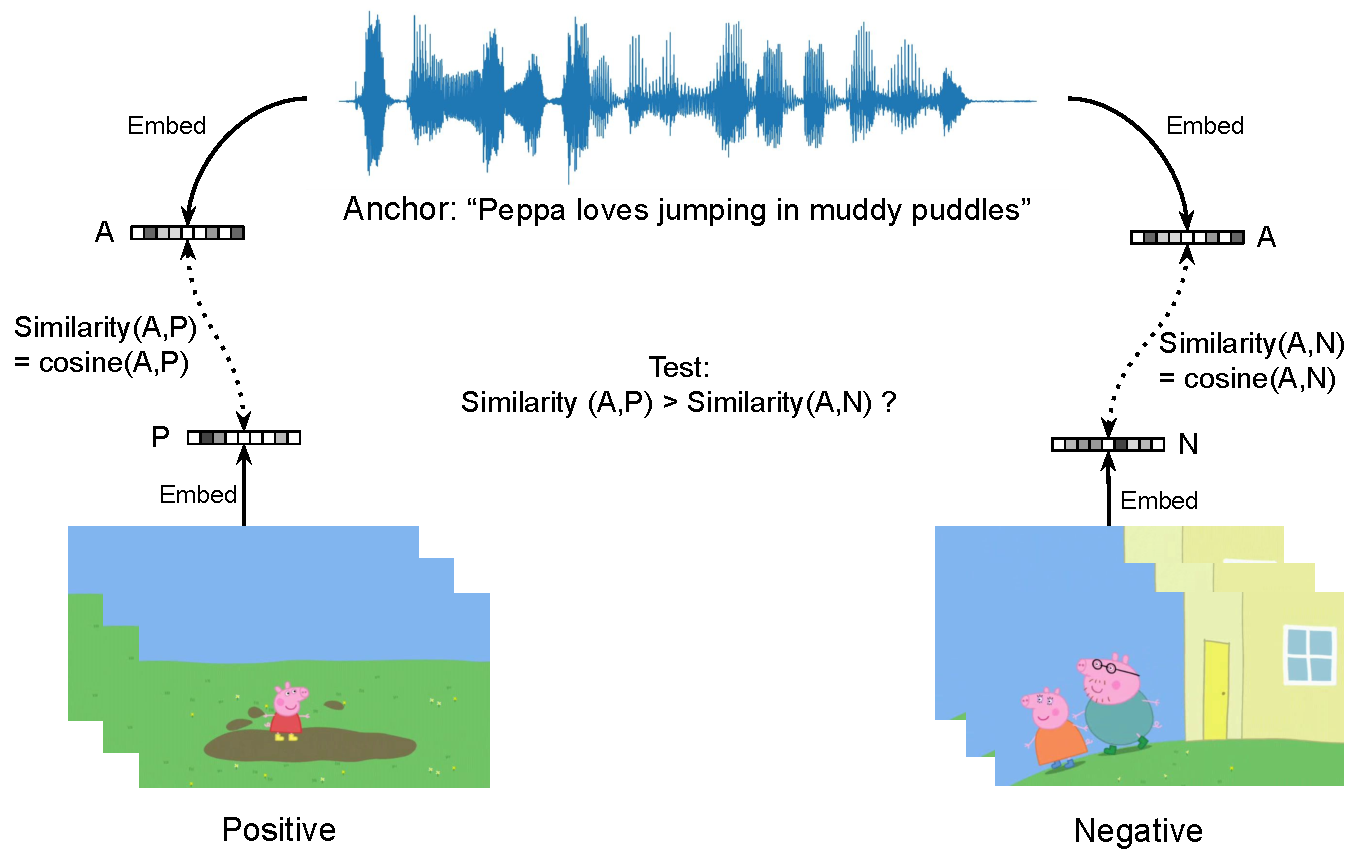
\includegraphics[width=\columnwidth]{peppa_triplets_eval_detailed.pdf}
	\caption{Triplets Evaluation: Given a reference audio sequence (anchor), we 
	measure the model's performance at choosing the matching video (positive) 
	over a random distractor video (negative).}
	\label{fig:triplets_eval}
\end{figure}

In our case, we extract clips aligned to a single subtitle
line, group them by length, and for each pair of same-length video
clips\footnote{To keep test items independent, the pairing of video
  clips is done such that each clip only occurs as a member of a single
  triplet.}, we extract the audio from one of them (selected at
random) -- this is our {\it anchor}. The video clip from which the
anchor was taken is the {\it positive} one, which the other video clip
is the {\it negative} one. This triplet of stimuli form a single test
item.  We use the model's audio encoder to encode the anchor, and the
video encoder to encode both video clips. We then check whether anchor
is more similar to the positive or negative clips in terms of cosine
similarity (see also \Cref{fig:triplets_eval}).  More precisely, {\it triplet 
accuracy} is the mean over
all triplets of the following quantity:
\begin{equation}
  \frac{\mathrm{signum}(\mathrm{cosine}(A, P) - \mathrm{cosine}(A, N)) + 1}{2}
  \label{eq:triplet-acc}
\end{equation}
with $A$ being the anchor, $P$ positive and $N$ negative. The triplet
accracy metric is inspired by the ABX score of \citet{schatz2016abx}.
For triplet accuracy, regardless of the specific set of test items, we
expect random-guessing performance to be at 0.5, and perfect
performance to be 1.0. For this metric we also quantify uncertainty by
resampling the triplets $500$ times from the dataset, and display the
score distribution.

\subsubsection{Minimal Pairs}
\label{sec:targeted}
While the triplet evaluation gives us a general idea about whether the model 
has learned a mapping between videos and audio, the metric does not provide 
insight into whether the model has acquired the grounded semantics of specific 
words.

To address this question, we probe the model's performance in a more targeted 
setup, where the model is not asked to rank the similarity of a correct video 
over a random video, but instead over a distractor video with \textit{minimal 
differences}.

More specifically, this approach considers always pairs of 
triplets with minimal differences regarding one word in the transcripts of
the anchor audios (e.g., \textit{Peppa loves jumping} and
\textit{George loves jumping} can be used to test whether the model
can discriminate the target word \textit{Peppa} from the distractor
word \textit{George}).

We search the transcripts of the validation data for phrases with
minimal differences with respect to the most commonly occurring (at least 10 
times) nouns, verbs, and adjectives. We set the minimum phrase duration to 0.3 
seconds (for shorter sequences, we do not expect that the video data contains 
enough semantic information for a model to distinguish between target and 
distractor). A phrase can also be a single word.


Based on each pair of phrases, we create two counter-balanced test trials, an 
example and a corresponding counter-example, as depicted in
\Cref{fig:minimal_pairs}. Here, 
the anchor $A_{\text{example}}$ of the example
triplet is the audio of \textit{Peppa loves jumping}, the
positive video $P_{\text{example}}$ is the corresponding video, and the
negative video $N_{\text{example}}$ is the video corresponding to \textit{George
  loves jumping}. In the
counter-example triplet, the anchor $A_{\text{counterex}}$ is the audio of
\textit{George loves jumping}, and the positive and negative video are
flipped: $P_{\text{counterex}} = N_{\text{example}}; N_{\text{counterex}} = P_{\text{example}}$. By 
evaluating the model on the examples as well as their corresponding 
counterexamples, we control the evaluation for linguistic biases in the dataset 
and ensure that a single-modality model that only considers the audio performs 
at chance \citep[see also][]{nikolaus-fourtassi-2021-evaluating}.

\begin{figure}[ht]
  \centering
  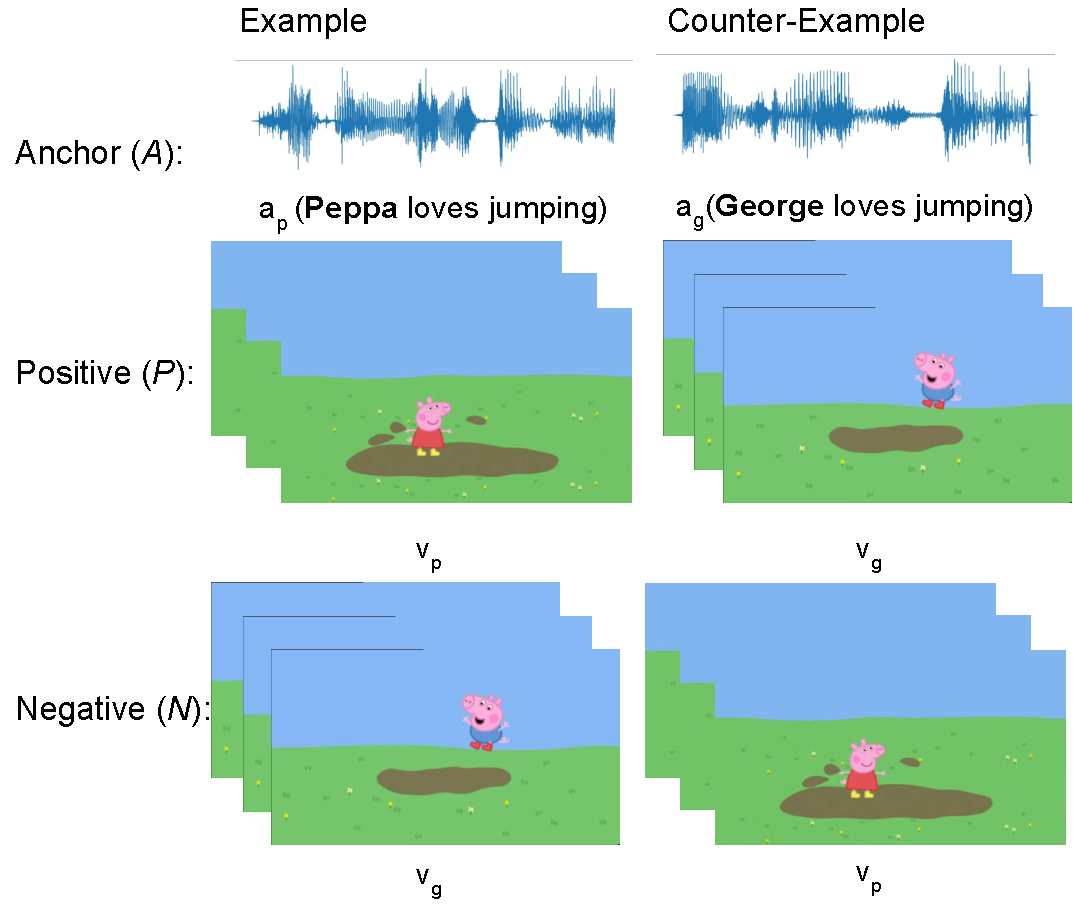
\includegraphics[width=\columnwidth]{peppa_targeted_triplets.pdf}
  \caption{Minimal Pairs Evaluation}
  \label{fig:minimal_pairs}
\end{figure}

We measure the model's accuracy for all examples and counter-examples using
\Cref{eq:triplet-acc} . Additionally, we report per-word accuracy by
calculating the triplet accuracy for all triplets that contain a given
word (e.g.\ \textit{Peppa}) either as target or distractor word, i.e.\ cases
in which the model needs to succeed in either choosing a video
containing the given word (the example triplet in Figure
\ref{fig:minimal_pairs}) or rejecting a video containing the given
word (the counter-example triplet in Figure
\ref{fig:minimal_pairs}).
%\footnote{In this way, both the example and the counter-example shown in 
%Figure \ref{fig:minimal_pairs} are also used to assess the acquisition of the 
%word ``George''.} 
We report accuracy for all words (nouns and verbs) for which we found at least 
100 example-counterexample pairs of triplets. There were not enough examples 
for adjectives in the dataset to perform an evaluation on them. 



\subsection{Model Architecture}
\label{sec:model}
We adapt the high-level modeling approach from work on spoken
image-caption data
\citep{harwath2016unsupervised,chrupala-etal-2017-representations}:
our objective function is based on a triplet-like contrastive loss with margin which
encourages the matching audio and video clip to be projected nearby in
the embedding space, and mis-matching audio and video clips to be far
away:
\begin{dmath}
  \ell = \sum_{av}\left[\sum_{a'} \max(0, S_{a'v} - S_{av} +
    \alpha) + \sum_{v'} \max(0, S_{av'} - S_{av} + \alpha) \right]
  \label{eq:triplet}
\end{dmath}
where $\alpha$ is a margin, $S_{av}$ is a similarity score between a
matching audio-video clip pair, and $S_{a'v}$ and $S_{av'}$ denote
similarity scores between mismatched pairs, i.e.\ negative examples
from the current batch. Our heuristic to generate positive and
negative examples is very simple: we consider the example
positive if the audio is aligned with a video clip in our
data. Other pairs of audio-video clips are considered negative.

\subsubsection{Audio Encoder}
The audio encoder portion of the model consists of a {\tt small
  wav2vec2} model \citep{wav2vec2} pre-trained in a self-supervised
fashion, without any supervised fine tuning.\footnote{Available from
  \url{https://dl.fbaipublicfiles.com/fairseq/wav2vec/wav2vec_small.pt}.}
The \textsc{wav2vec 2.0} architecture learns audio embeddings by
self-supervised learning driven by a contrastive loss applied to 
quantized latent representations of masked frames, loosely inspired by
the BERT approach to language modeling \citep{devlin-etal-2019-bert}.

The output of this module is a temporal sequence of 28-dimensional vectors. We
pool this output across time using an attention mechanism with
dimension-wise weights \citep{Merkx2019}:
\begin{equation}
  \begin{aligned}
    \mathbf{A} = & \mathrm{softmax}_t\left(\mathrm{MLP}(\mathbf{X})\right)\\
    \mathbf{z} = & \sum_t \left( \mathbf{A}_{t} \odot \mathbf{X}_{t} \right),
  \end{aligned}
  \label{eq:att-pool}
\end{equation}
where $\mathbf{X}$ is the tensor with the encoder output vectors for
each time-step: an MLP followed by a time-wise
softmax is used to compute an attention weight for each time step and for each
dimension.
%Each dimension of the pooled embedding vector $\mathbf{z}$
%consists of a weighted sum across time of the output values at this
%dimension.
The pooling is followed by a linear projection and $L_2$
normalization. For our experiments we also use versions of the encoder
where the wav2vec weights are frozen, as well a randomly initialized
rather than pre-trained.



\subsubsection{Video Encoder}
As a video encoder we use the 18-layer ResNet (2+1)D architecture
\citep{tran2018closer} pretrained on the action recognition dataset
Kinetics-400 \citep{DBLP:journals/corr/KayCSZHVVGBNSZ17}. The
pre-trained model is available via Pytorch.\footnote{See
  \url{https://pytorch.org/vision/0.8/models.html\#resnet-3d}.}  This
architecture implements 3D convolution by decomposing it into a 2D
spatial convolution followed by 1D temporal convolution.  The output
of this module is aggregated using the attention mechanism with the
same architecture as for the audio module, linearly projected to the
same dimensionality as the audio (512) and $L_2$ normalized.  For our
experiments we also use a version of the video encoder without
pre-training.

\paragraph{\textsc{Static} baseline}
As a baseline to investigate the contribution of temporal information to
video modeling we swap the video ResNet (2+1)D with the D2 ResNet
pre-trained on ImageNet, which embeds each video frame
separately. These frame embeddings are then attention-pooled as with
the standard video encoder. 


\section{Experimental Settings}
We implement the architecture in Pytorch \citep{NEURIPS2019_9015}. We
use the Adam optimizer \citep{kingma2014adam} with the scheduling
described in \citep{devlin-etal-2019-bert}. We train every
configuration on a single GPU and stop training after 48 hours, with
batch-size 8 and accumulating gradients over 8 batches, in 16 bit
precision mode. For each model configuration we save model weights
after each epoch and report results for the checkpoint which gets the
best triplet accuracy on the narration validation data.
Our code is publicly available at \url{github.com/gchrupala/peppa},
and can be consulted for further details of the experimental setup.

\section{Results}
\label{sec:results}
\paragraph{Performance metrics}


In the case of the narration data this scores is not confounded by
speaker-based clues, which is an indication that the model possibly
learned to detect some aspects of utterance meaning. 

\begin{figure*}[htb]
  \centering
  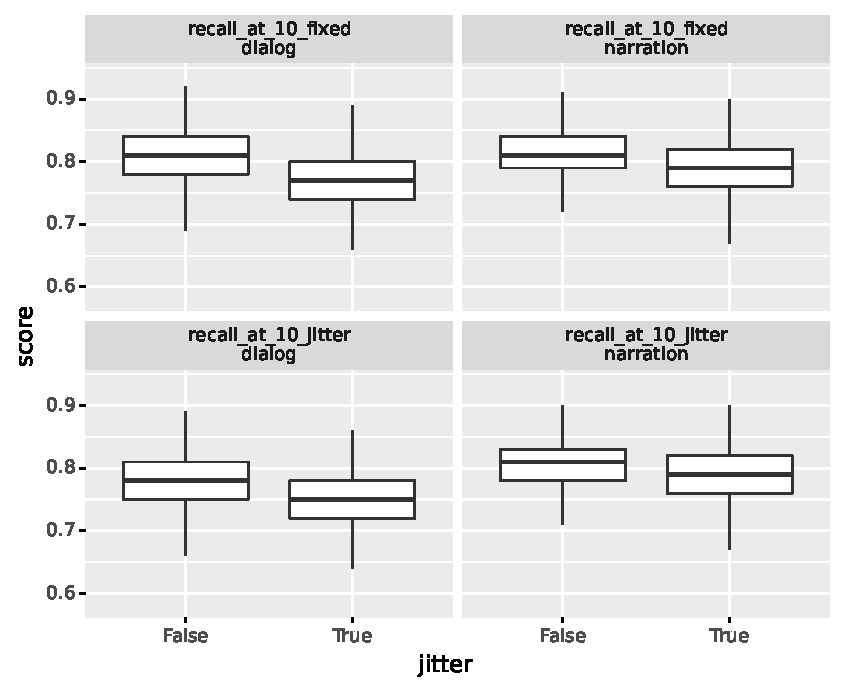
\includegraphics[width=0.9\textwidth]{results/ablations/jitter.pdf}
  \caption{Effect of jitter.}
  \label{fig:jitter}
\end{figure*}

\begin{figure*}[htb]
  \centering
  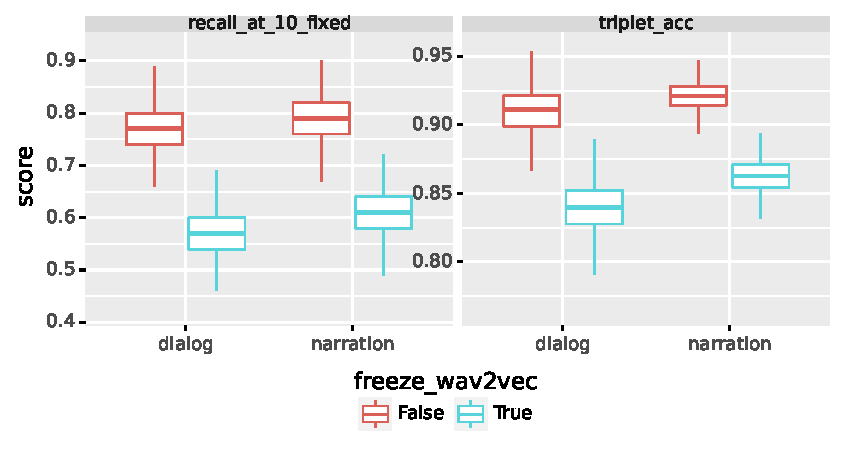
\includegraphics[width=0.9\textwidth]{results/ablations/freeze_wav2vec.pdf}
  \caption{Effect of freezing the parameters of the \textsc{wav2vec} module.}
  \label{fig:freeze_wav2vec}
\end{figure*}

\begin{figure*}[htb]
  \centering
  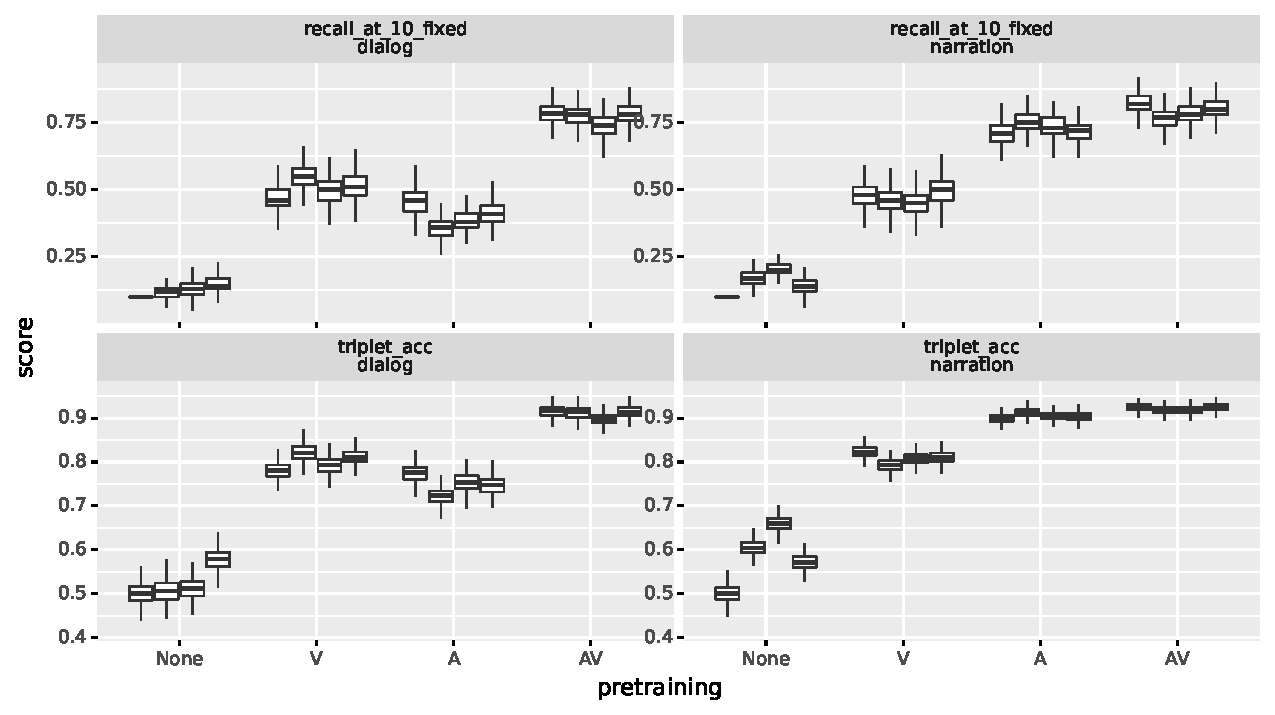
\includegraphics[width=0.9\textwidth]{results/ablations/pretraining.pdf}
  \caption{Effect of pre-training.}
  \label{fig:pretraining}
\end{figure*}

\begin{figure*}[htb]
  \centering
  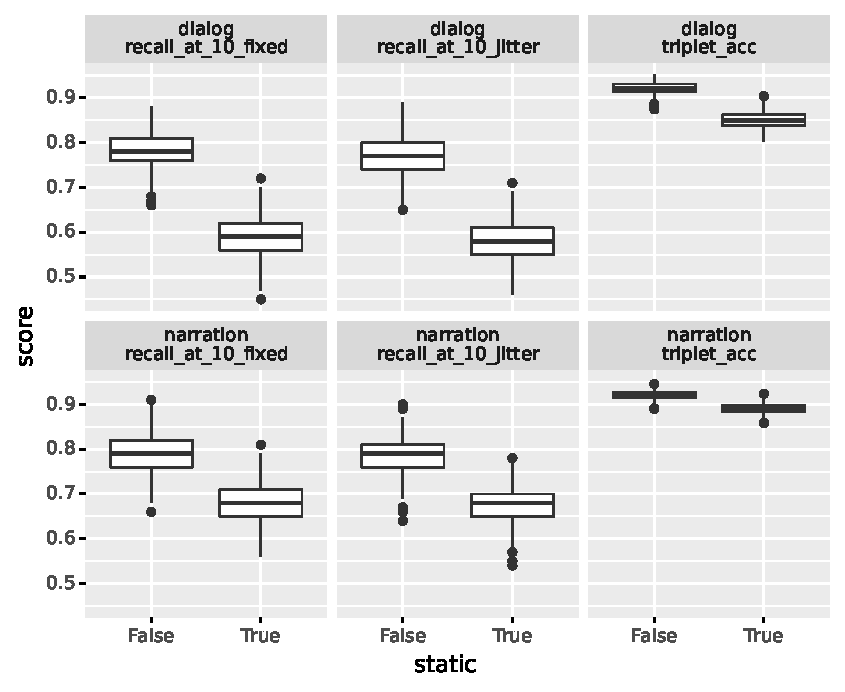
\includegraphics[width=0.9\textwidth]{results/ablations/static.pdf}
  \caption{Effect of temporal information.}
  \label{fig:static}
\end{figure*}


\paragraph{Minimal Pairs}
As a first baseline, we evaluate a model that has been pretrained but not fine-tuned on our dataset. The resulting performance is, as expected, close to chance level: 0.538.\todo{MN: add baselines: model that is completely untrained, and model where only the attention pooling layers are finetuned} Additionally, we evaluate a model that is trained using static (image) data instead of video. The average accuracy is 0.705 . Finally, the best performing model according to the
performance metrics (ID 68, audio and video pretraining) achieves an average
targeted triplets accuracy of 0.745.

\Cref{fig:accuracy_targeted_triplets_nouns} and
\ref{fig:accuracy_targeted_triplets_verbs} show per-word
accuracy for nouns and verbs, respectively. We perform boostrapping (n\_resampling = 100) to estimate mean and standard deviation for each accuracy score.

We further compute correlations between the per-word accuracy and two 
possible predictors of age of acquisition: frequency and concreteness. 
We do not find any significant correlation between the model's per-word 
accuracy and word concreteness or input frequency of a word in the 
training data.\todo{MN: verify correlations for final versions}




\begin{figure*}[htb]
  \centering
  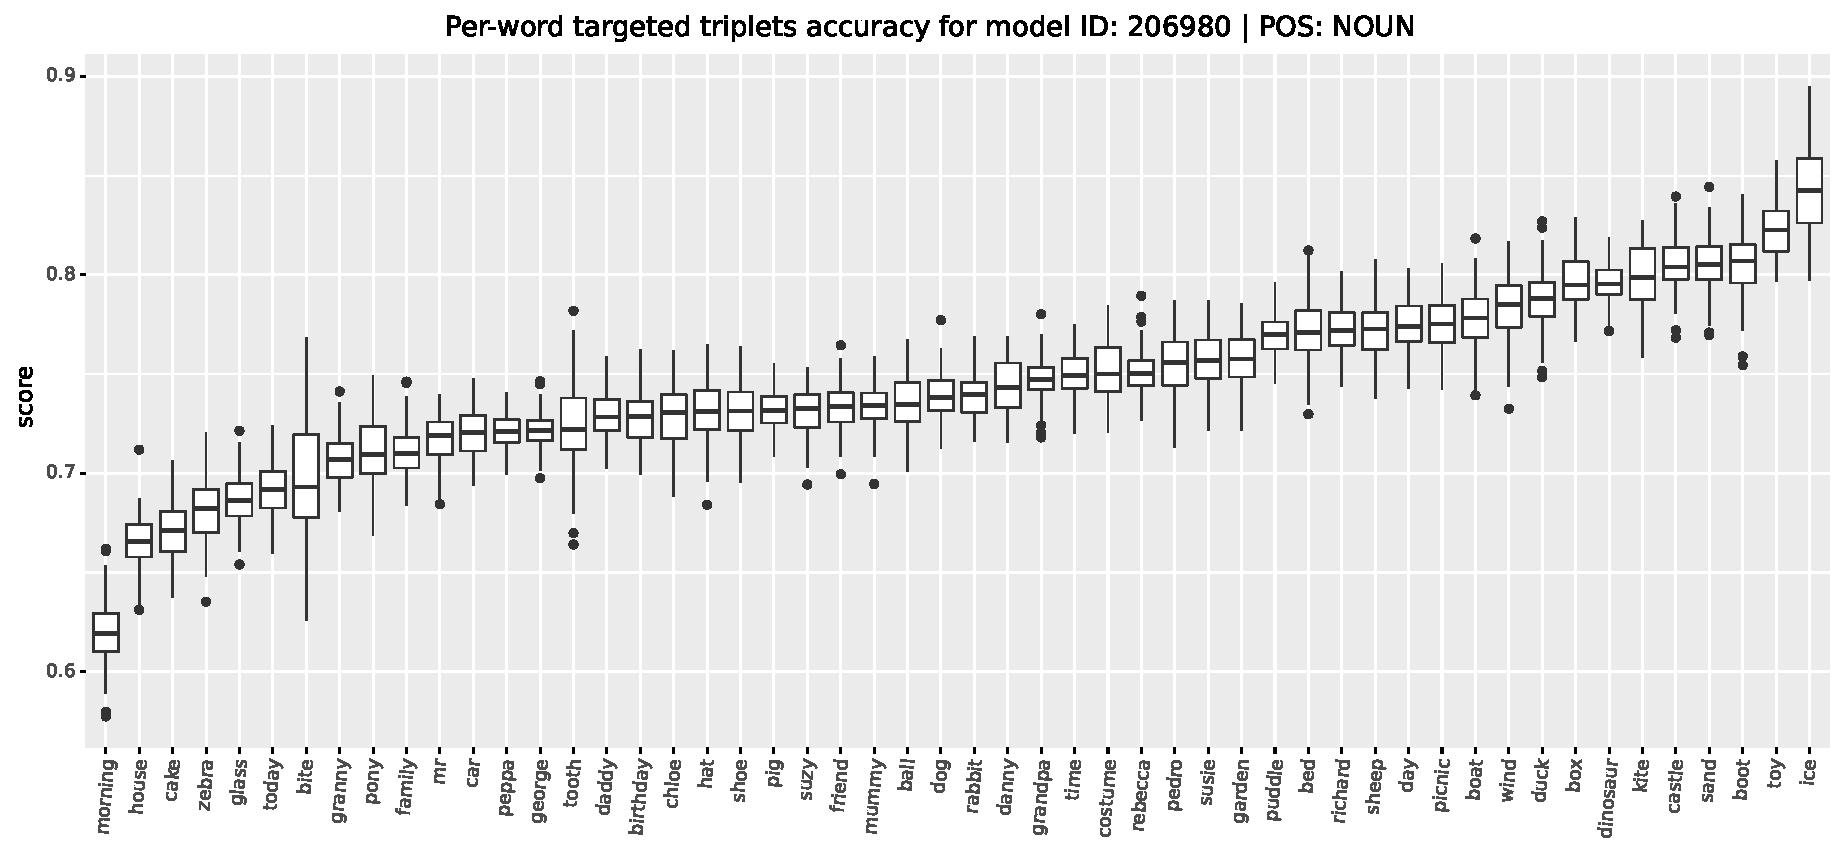
\includegraphics[width=\textwidth]{results/targeted_triplets/results_per_word_version_206980_NOUN.pdf}
  \caption{Per-word targeted triplets accuracy for nouns.}
  \label{fig:accuracy_targeted_triplets_nouns}
\end{figure*}

\begin{figure*}[htb]
  \centering
  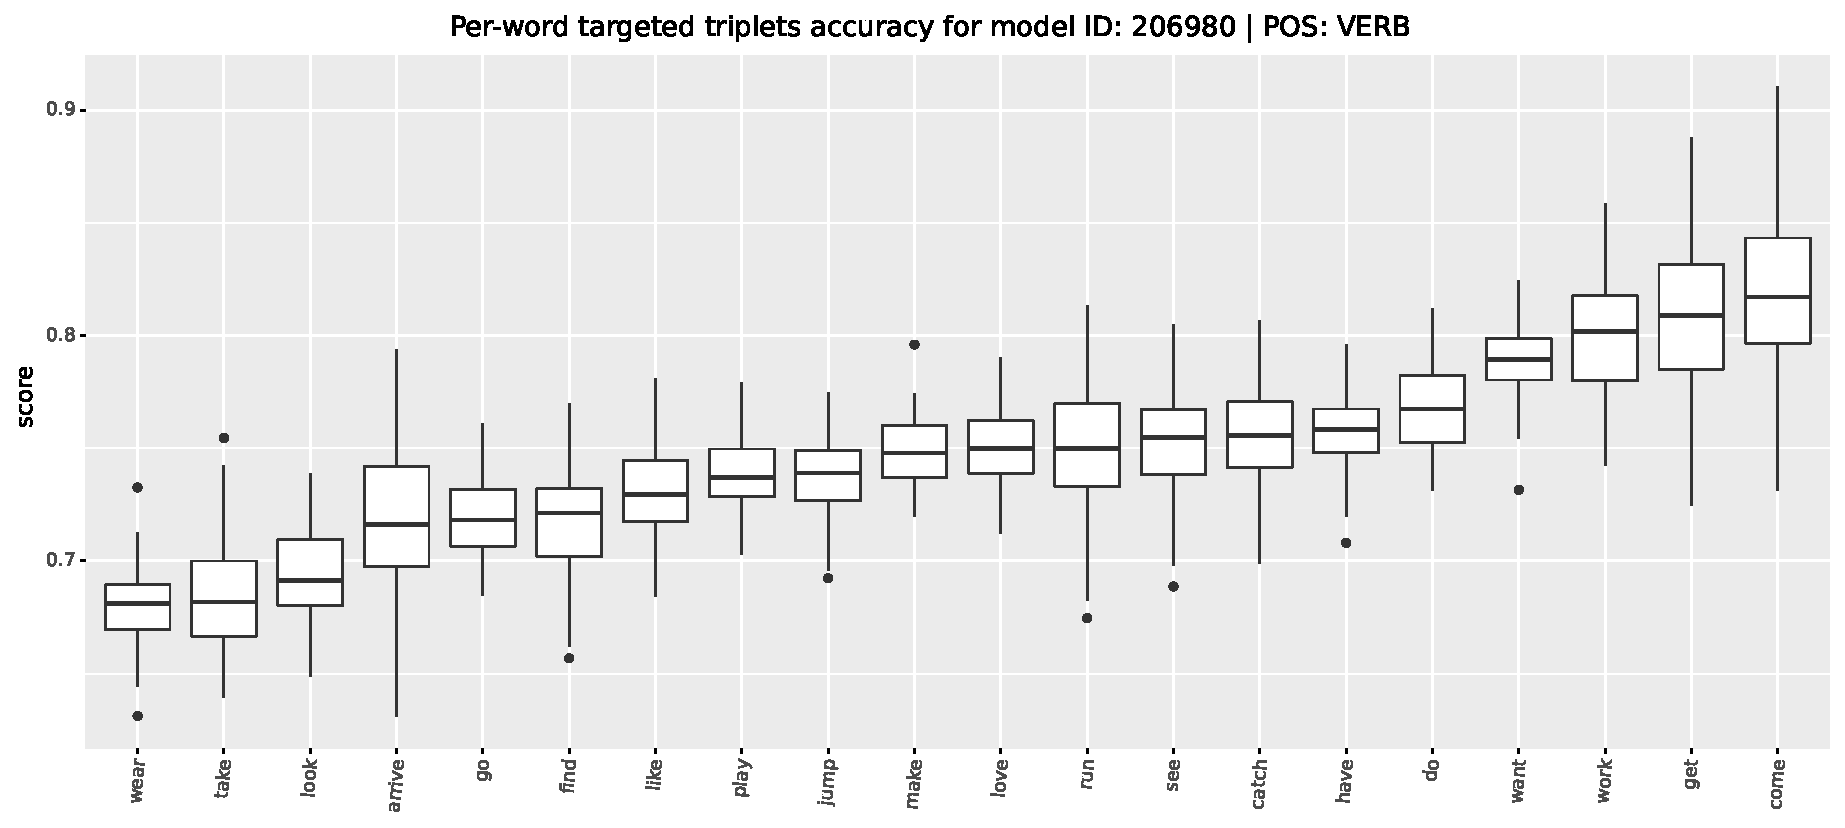
\includegraphics[width=\textwidth]{results/targeted_triplets/results_per_word_version_206980_VERB.pdf}
  \caption{Per-word targeted triplets accuracy for verbs.}
  \label{fig:accuracy_targeted_triplets_verbs}
\end{figure*}

\section{Conclusion}
\label{sec:conclusion}
Our results suggest that despite the challenges inherent to the
naturalistic aspects of the \emph{Peppa Pig} dataset, a simple bimodal
architecture trained on it captures aspects of visual meaning of individual 
words as well as full utterances, and generalizes well to narrative utterances
featuring a single unseen speaker and a descriptive rather than
conversational style. We saw that generalization is substantially
boosted by fine-tuning audio representations pretrained on unlabeled
single-modality speech data. Fine-tuning a pretrained video encoder
also makes a contribution, but is less crucial to generalization from
dialog to narration.


\subsection{Limitations and Future Work}
\label{sec:limitations}
We model the acquisition of spoken language from both
language-internal correlations as well as from grounding in vision in
a simplistic way: we fine-tune an audio encoder pretrained on read
speech.
In future, it would be interesting to make the setting
more realistic by using pretraining data which reflect a young
learner's experience more closely, and to realistically interleave learning via
self-supervision from speech and via grounding in vision.
Ideally we would also want to dispense with
supervised pretraining of the video encoder and rather use a model pretrained in a
self-supervised way also for this modality.

In order to investigate what aspects of spoken language our model
acquires, we would like to carry out in-depth analyses of learned 
representations on sub-word, lexical, and phrasal levels. It would also be 
worthwhile to figure out the details of how specifically temporal information 
in video contributes to acquiring linguistic knowledge. While some analyses in 
this direction were currently constrained by the size of the evaluation 
dataset, in the future one could apply similar methods on more large-scale data.

Using naturalistic datasets such as the \textit{Peppa Pig} cartoons, we belief 
that it will be possible relate findings more closely to theories in 
language acquisition in the real world.



\bibliography{biblio,anthology}
\bibliographystyle{acl_natbib}
\appendix

\section{Supplementary material}

\subsection{Retrieval and triplet accuracy}
\Cref{tab:scores-dialog} and \Cref{tab:scores-narration} show
the performance of several model configurations on the retrieval and
triplet tasks on the dialog and narration datasets respectively.
\todo{GC: Tables out of date}
 \begin{table*}[htb]
   \centering
   \begin{tabular}{rlrr}
\toprule
 ID & Pretraining &  Recall@10 &  Triplet Acc \\
\midrule
 43 &          AV &      0.193 &        0.814 \\
 44 &           V &      0.084 &        0.728 \\
 45 &        None &      0.034 &        0.597 \\
\bottomrule
\end{tabular}

   \caption{Retrieval and triplet scores on dialog validation data.}
   \label{tab:scores-dialog}
 \end{table*}

\begin{table*}[htb]
   \centering
   \begin{tabular}{rlrr}
\toprule
 ID & Pretraining &  Recall@10 &  Triplet Acc \\
\midrule
 43 &          AV &      0.239 &        0.866 \\
 44 &           V &      0.166 &        0.822 \\
 45 &        None &      0.087 &        0.741 \\
\bottomrule
\end{tabular}

   \caption{Retrieval and triplet scores on narration validation data.}
   \label{tab:scores-narration}
 \end{table*}

\subsection{Targeted Triplets Evaluation Sets}\label{app:targeted_triplets_eval}

To find commonly occurring nouns, adjectives, and verbs, we lemmatize and POS-tag all words in the transcripts of the validation dataset using spacy \citep{honnibal2020spacy}. Afterwards, we identify sets of all nouns $\{n_1, ..., n_n\}$, verbs $\{v_1, ..., v_o\}$ and adjectives $\{a_1, ..., a_p\}$ that occur at least 10 times in the validation data. Given these sets, we create sets of tuples $\{(n_1, n_2), (n_1, n_3), ..., (n_1, n_n), ...,  (n_{n-1}, n_n)\}$ for all combinations of nouns and verbs, respectively. For each of these tuples, we search the validation data for pairs of phrases $(p_k=[w_1, ..., w_x], p_l=[w_1, ..., w_y])$ with same length ($x=y$) and minimal difference regarding the tuple. That is, $n_1 \in p_1$, $n_2 \in p_2$, and if we replace $n_1$ with $n_2$ in $p_1$, it is equal to $p_2$. 

For example, if $n_1 = \text{"peppa"}$ and $n_2 = \text{"george"}$, the phrases $p_1 = [\text{"peppa", "loves", "jumping"}]$ and $p_2 = [\text{"george", "loves", "jumping"}]$ are phrases with minimal differences. A phrase can also be a single word.

We set the minimum phrase duration to 0.3 seconds (for shorter sequences, we do not expect that the video data contains enough semantic information for a model to distinguish between target and distractor). For each phrase $p_1$ we look for the \textit{longest} possible phrase $p_2$. \Cref{fig:num_samples_vs_duration} shows the distribution of samples per duration.

Based on each minimal pair, we construct two counter-balanced test triplets as described in the main text.

Figures \ref{fig:num_samples_NOUN_word}, and \ref{fig:num_samples_VERB_word} show the number of samples for each noun and verb for which at least 100 sets of test triplets were available (for no adjective there were enough samples found).


\begin{figure}
  \centering
  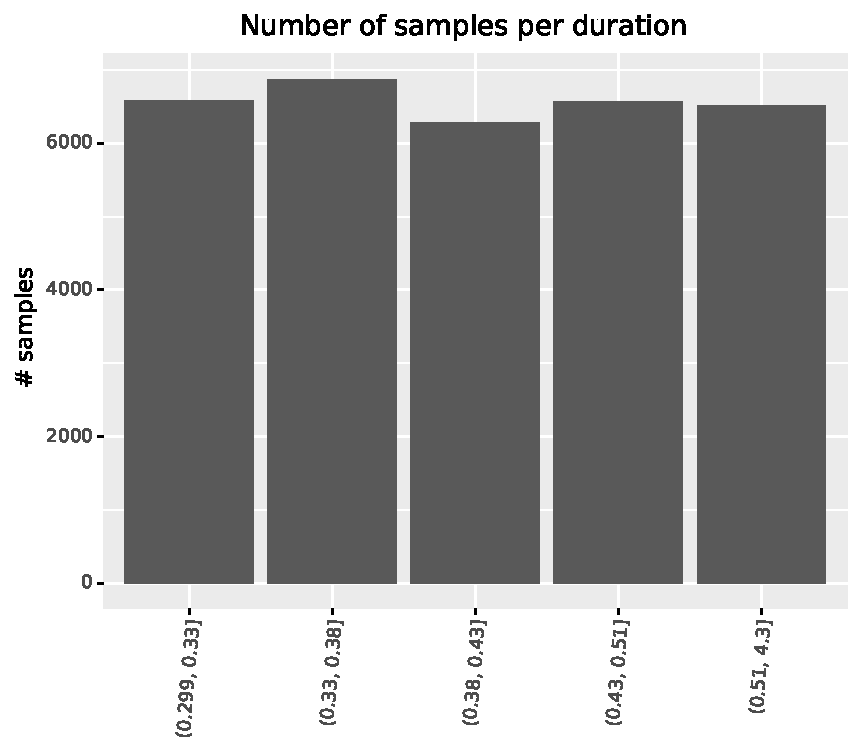
\includegraphics[width=\columnwidth]{results/targeted_triplets/num_samples_per_duration.pdf}
  \caption{Number of samples per duration}
  \label{fig:num_samples_vs_duration}
\end{figure}


\begin{figure*}
  \centering
  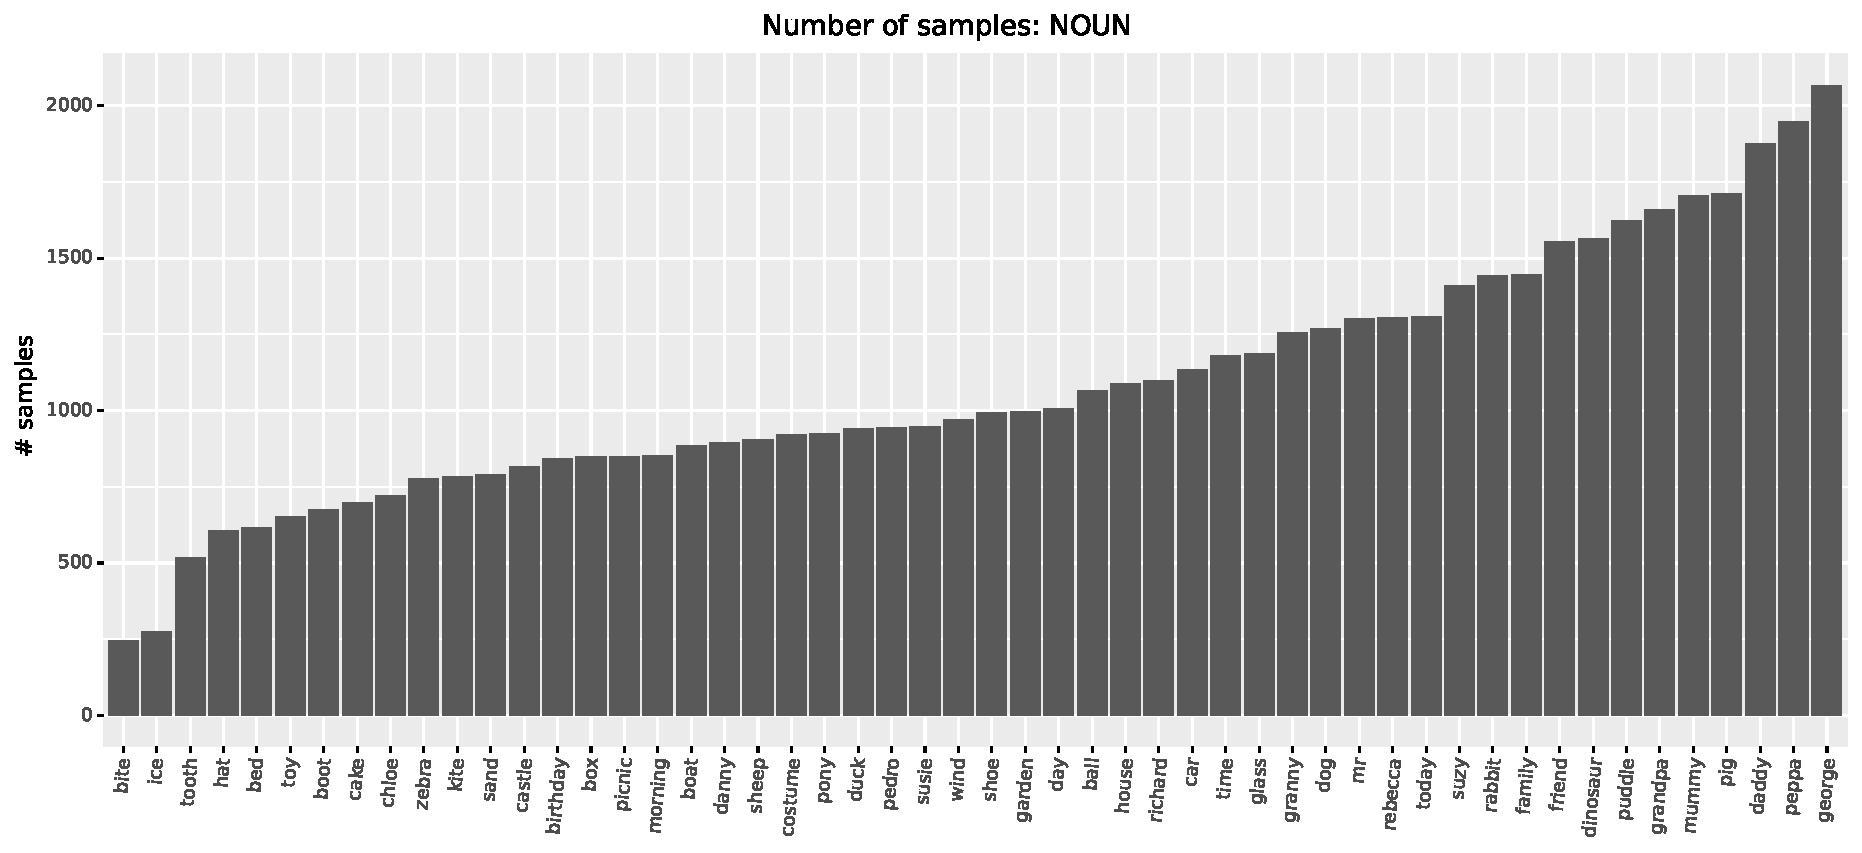
\includegraphics[width=\textwidth]{results/targeted_triplets/num_samples_per_word_NOUN.pdf}
  \caption{Number of samples: nouns}
  \label{fig:num_samples_NOUN_word}
\end{figure*}

\begin{figure*}
  \centering
  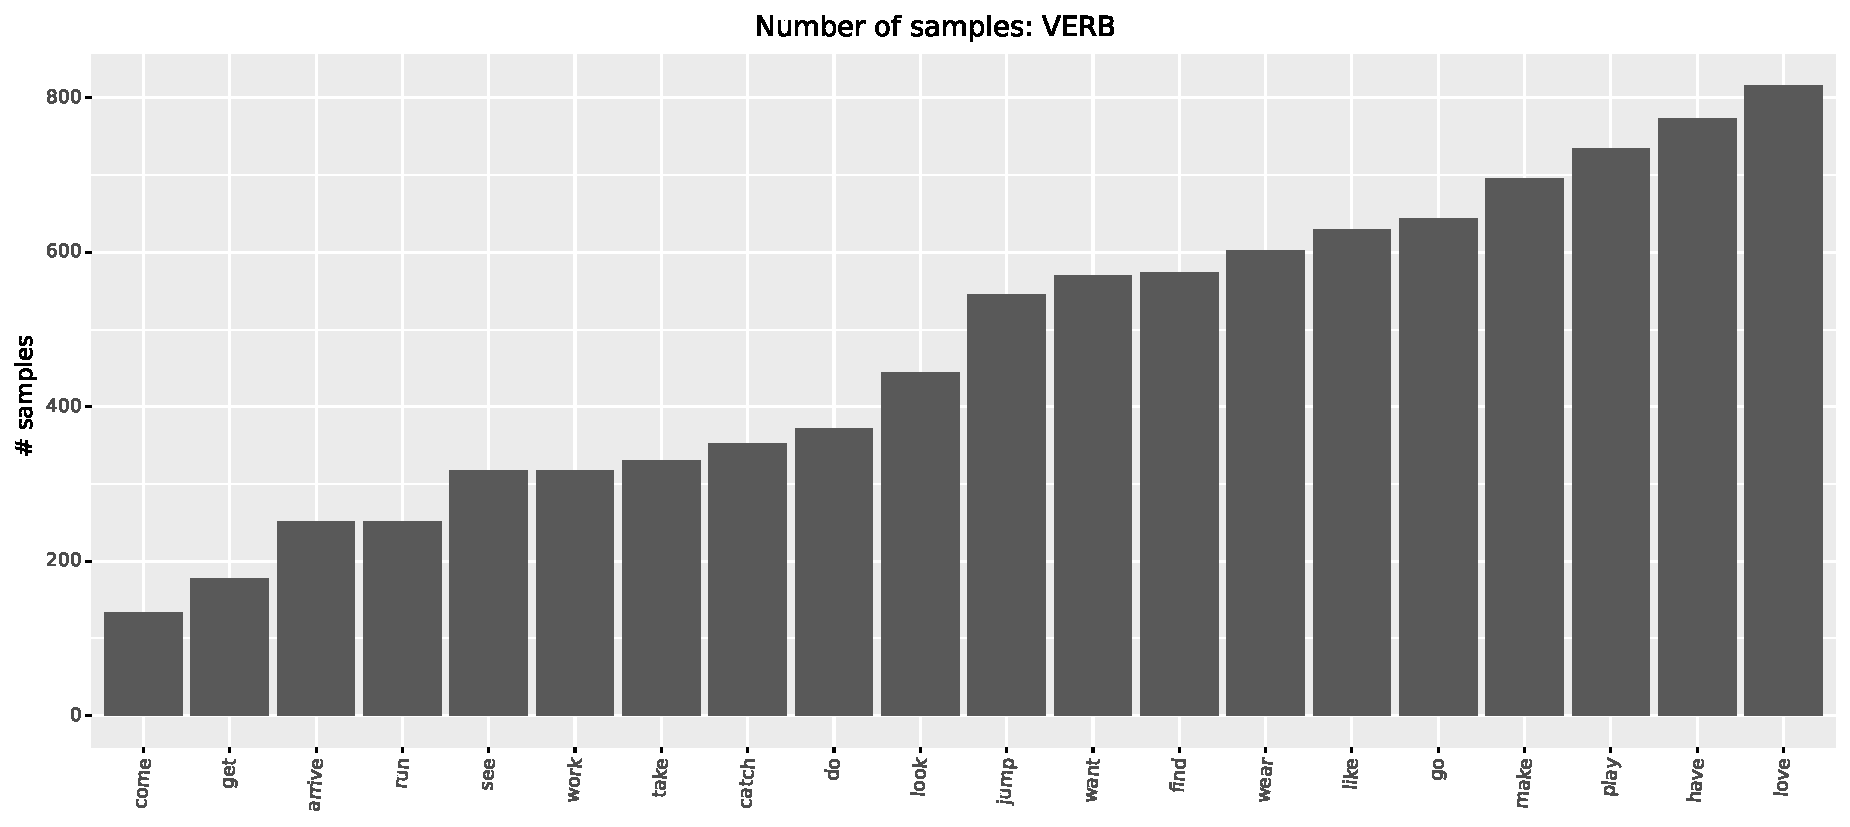
\includegraphics[width=\textwidth]{results/targeted_triplets/num_samples_per_word_VERB.pdf}
  \caption{Number of samples: verbs}
  \label{fig:num_samples_VERB_word}
\end{figure*}

\subsection{Targeted Triplets Correlations}\label{app:targeted_triplets_correlations}

\Cref{fig:results_correlation_frequency_acc} shows the correlation between per-word accuracy and frequency of this word in the training data.
\Cref{fig:results_correlation_concreteness_acc} shows the correlation between per-word accuracy and concreteness scores.


\begin{figure}
  \centering
  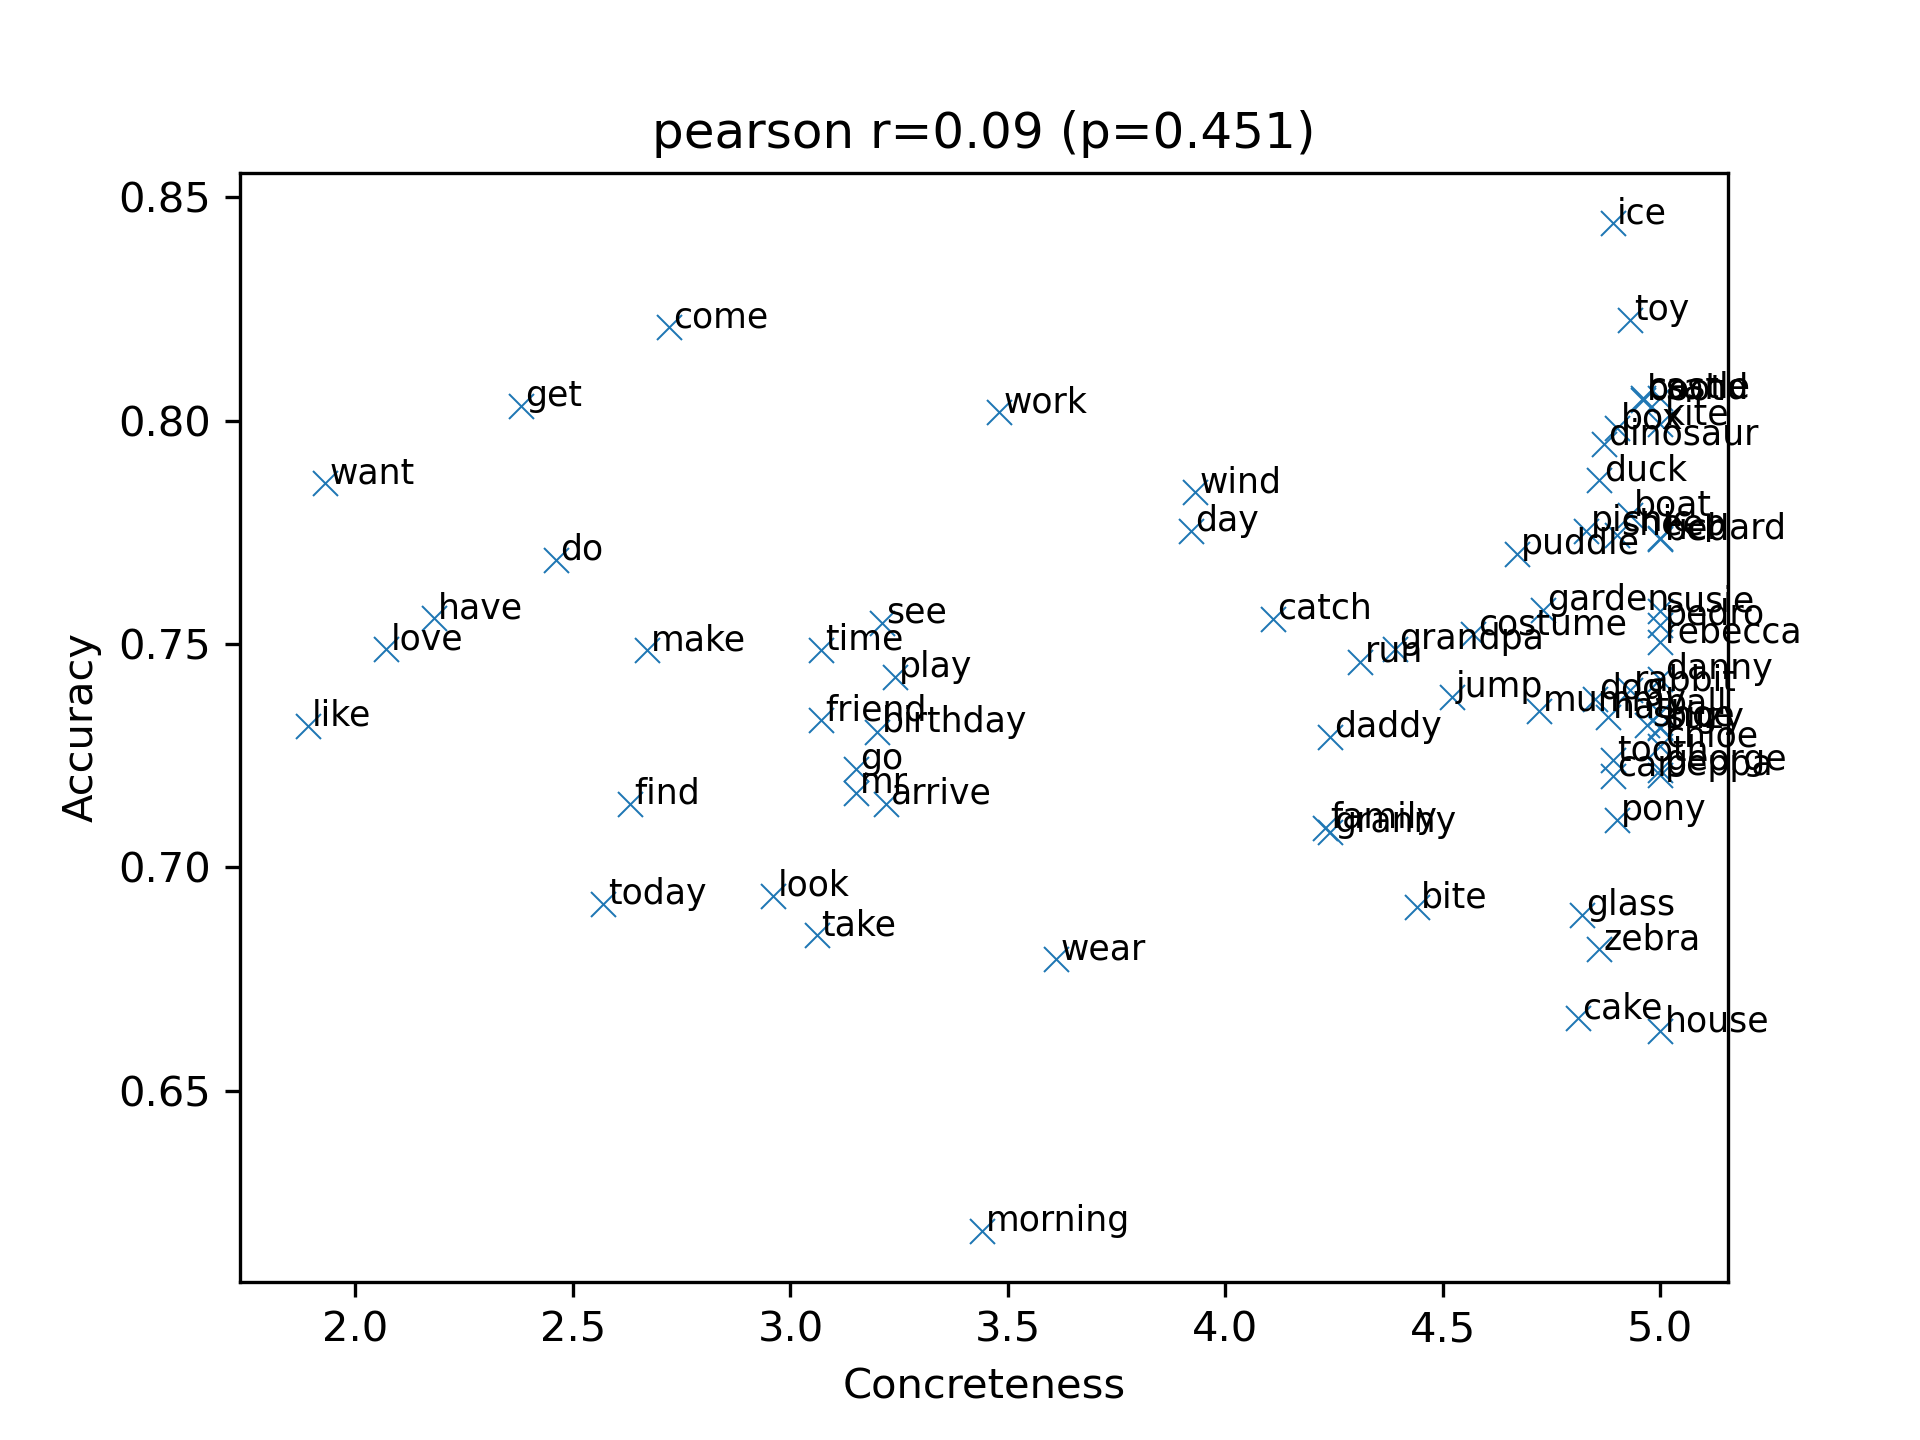
\includegraphics[width=\columnwidth]{results/targeted_triplets/correlation_concreteness_acc_version_206980.png}
  \caption{Correlation between accuracy and log frequency.}
  \label{fig:results_correlation_frequency_acc}
\end{figure}

\begin{figure}
  \centering
  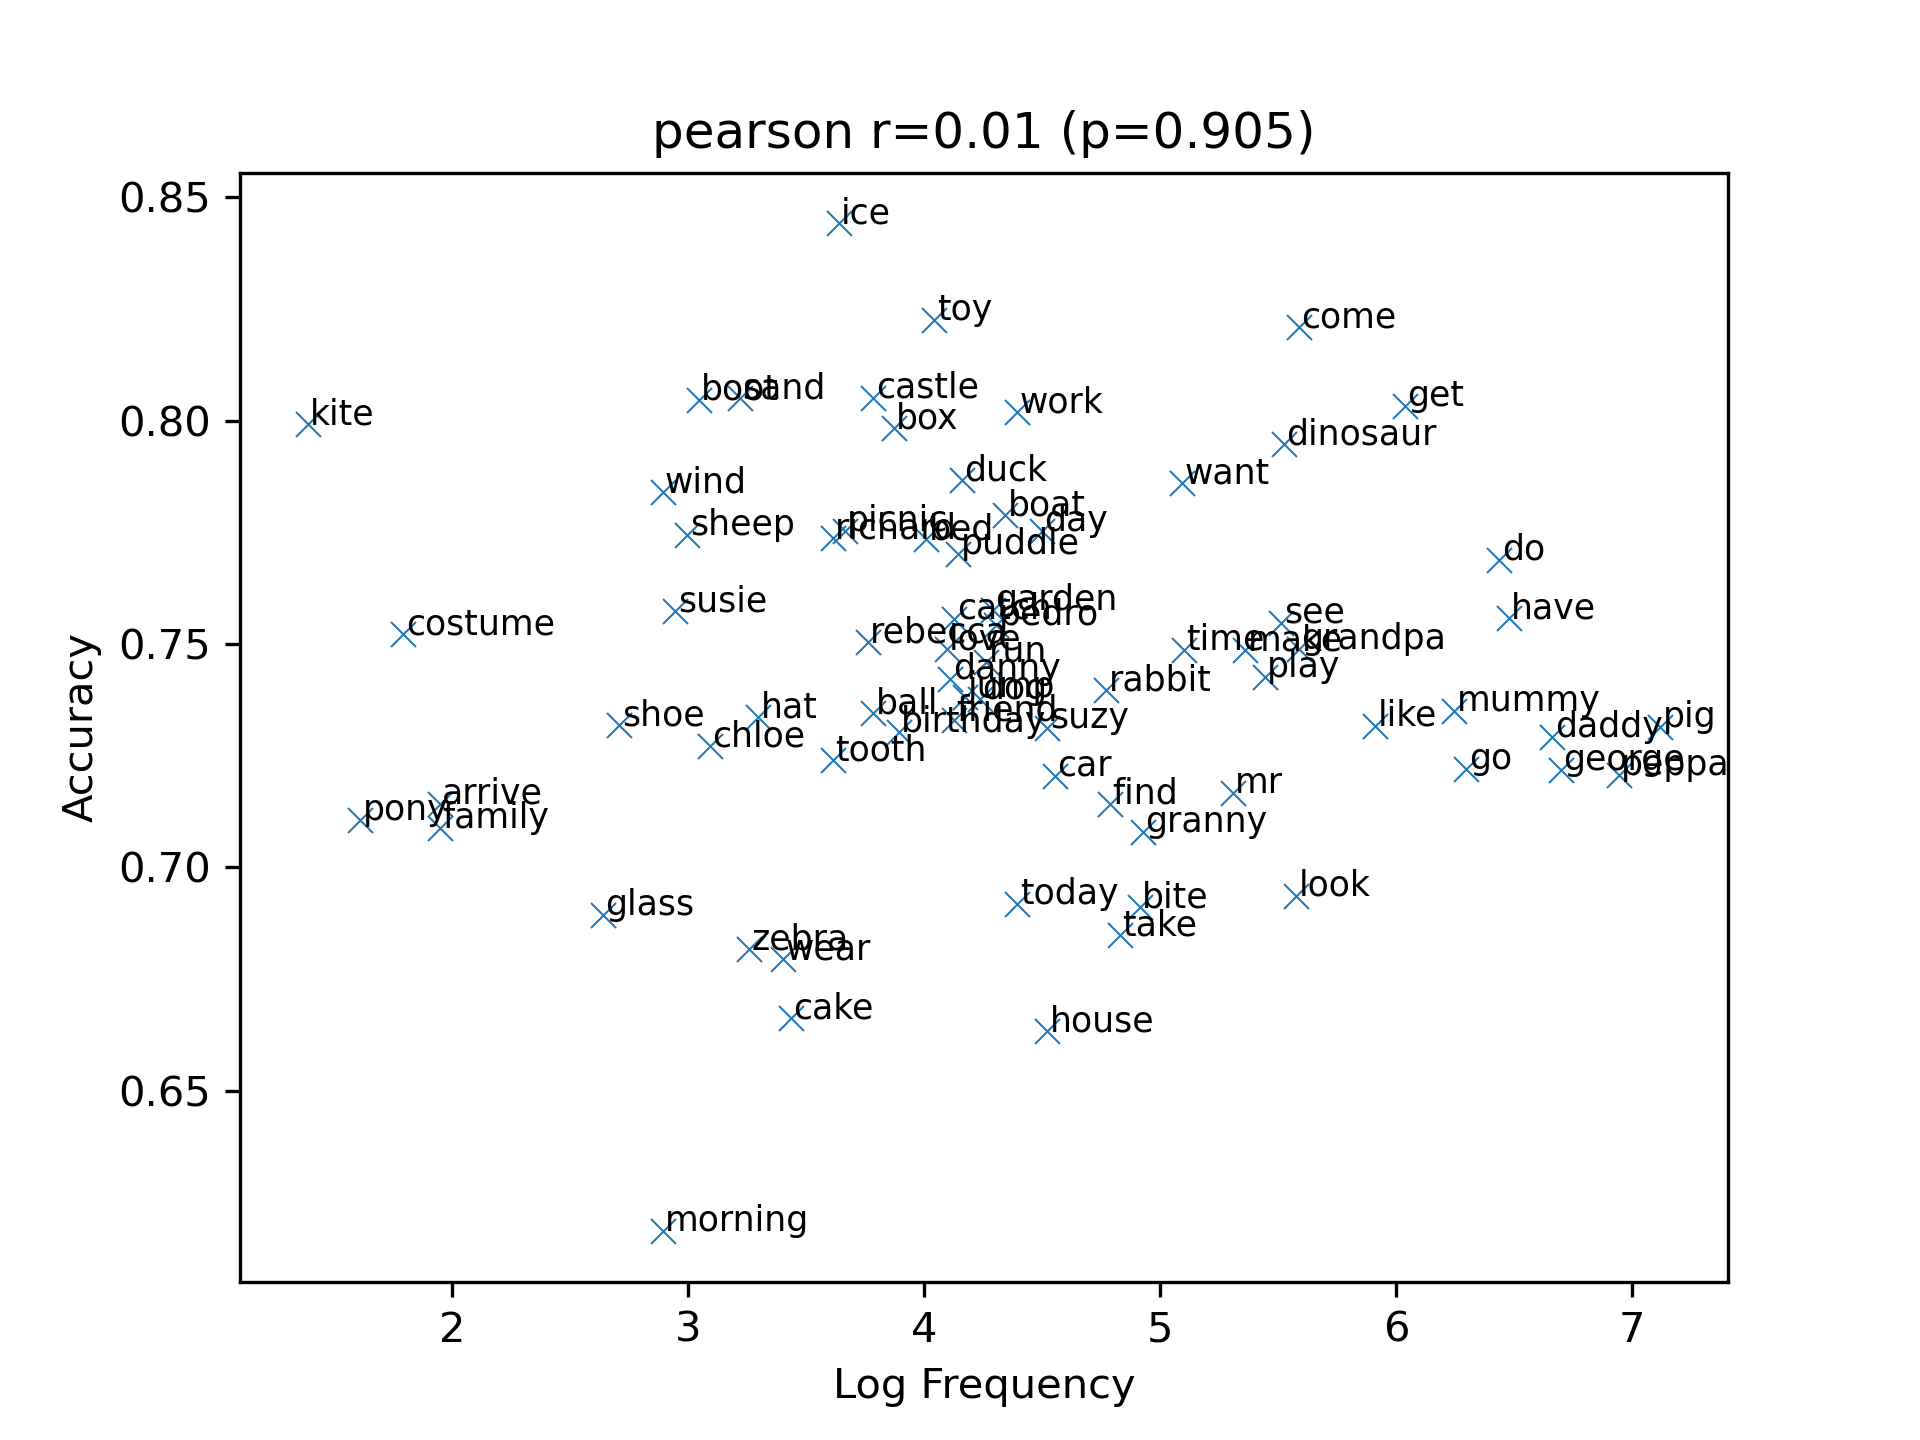
\includegraphics[width=\columnwidth]{results/targeted_triplets/correlation_frequency_acc_version_206980.png}
  \caption{Correlation between accuracy and concreteness.}
  \label{fig:results_correlation_concreteness_acc}
\end{figure}


\end{document}
